%%%
% Denne fil indeholder noter til Kontekstfrie Sprog (Kapitel 2 i Sipser)
% Derudover indeholder den også mine løsninger til opgaver om kontekstfrie sprog.
% Opgaver:
% TODO: Kapitel 2.2
% TODO: Kapitel 2.3
%%%
\chapter{Kontekstfrie Sprog}

\index{Kontekstfri Grammatik}
\index{Kontekstfri Sprog!Defineret}
I det tidligere kapitel om endelige automater, så vi den klasse af sprog som de genkender, regulære sprog, men vi så også eksempler på sprog som ikke er regulære, og hvordan dette kan bevises. I dette kapitel vil vi introducere \textit{kontekstfrie grammatikker} som er stærkere end endelige automater i deres deskriptionskraft. Sprogene der genkendes af kontekstfrie grammatikker kaldes \textit{kontekstfrie sprog}. Ydermere introducerer vi \textit{stakautomater} (pushdown automata på engelsk) som er en klasse af maskiner der genkender kontekstfrie sprog.

Et sprog kaldes \textit{kontekstfri}, fordi dets udledning\footnote{Definition for udledning  er i starten af Sektion~\ref{sec:cfg}} \textit{ikke} afhænger af dens kontekst, e.g., hvis du erstatter $A$ i $uAv$ så er det ikke afhængigt af $u$ eller $v$.

\section{Kontekstfrie Grammatikker}
\label{sec:cfg}
\index{Produktioner}
En grammatik består af en samling af \textbf{substitueringsregler}, også kaldet \textit{produktioner}. Hver regel forekommer som en linje i grammatikken,  og består af et symbol efterfulgt af en pil efterfulgt af en streng. Følgende grammatik er et eksempel på en kontekstfri grammatik $G_{1}$:
\begin{equation}
	\tag{$G_{1}$}
	\begin{split}
		A &\rightarrow \mathtt{0}A \mathtt{1}\\
		A &\rightarrow B\\
		B &\rightarrow \mathtt{\#}
	\end{split}
	\label{eqn:G1}
\end{equation}

\index{Variabel}
\index{Terminal}
Symbolet på venstresiden kaldes en \textit{variabel}\footnote{Kært barn har mange navne, jeg har også hørt non-terminal og, simpelt, LHS.}. Strengen (højresiden) består af variabler og andre symboler, kaldet \textit{terminale}. Terminale minder om alfabetet fra en endelig automat, da disse er de endelige symboler, der udgør en resulterende streng\footnote{Dette vil vi komme ind på i mere detalje senere.}. Variabler er oftest repræsenteret som store bogstaver, hvor terminale kan være små bogstaver, tal, eller specielle symboler (såsom \#.) En af variablerne (venstrehåndssiden) bliver udpeget til at være \textbf{startvariablen}. Denne variabel skal alle udledninger af grammatikken starte på (analogt til en start state i en endelig automat.)

\index{Udledning}
For at beskrive et sprog med en grammatik, \textit{udleder} vi strenge fra grammatikken. Dette bliver gjort systematisk ved at \textit{substituere} variabler med andre variabler eller terminale. Eksempeltvis kan gramatikken \ref{eqn:G1} udlede strengen \texttt{000\#111}. En udledning af denne streng i \ref{eqn:G1} er følgende: $A \Rightarrow \mathtt{0}A \mathtt{1} \Rightarrow \mathtt{00}A \mathtt{11} \Rightarrow \mathtt{000}A \mathtt{111} \Rightarrow \mathtt{000}B \mathtt{111} \Rightarrow \mathtt{000\#111}$. En måde hvorpå du kan vise dette grafisk er \textit{parse-træer}. Et eksempel kan ses i Figur~\ref{fig:parsetreeg1}, som viser et parsetræ for strengen \texttt{000\#111} i grammatikken \ref{eqn:G1}.
\index{Træ!Parse}
\begin{figure}[ht]
	\centering
	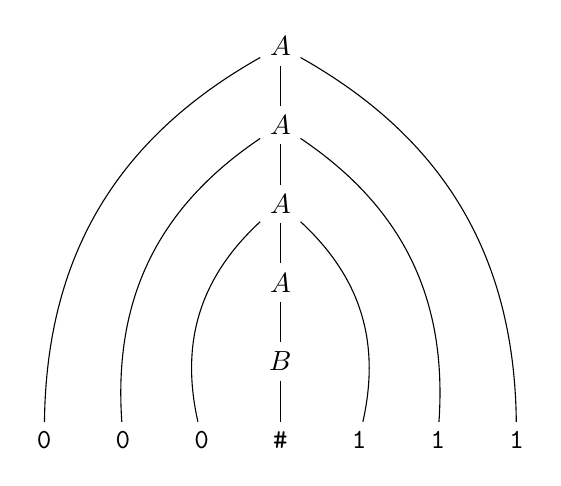
\begin{tikzpicture}[>=latex]
		% Nodes
		\node (0a) at (0,0) {\texttt{0}};
		\node (0b) at (1,0) {\texttt{0}};
		\node (0c) at (2,0) {\texttt{0}};
		\node (sharp) at (3,0) {\texttt{\#}};
		\node (1a) at (4,0) {\texttt{1}};
		\node (1b) at (5,0) {\texttt{1}};
		\node (1c) at (6,0) {\texttt{1}};

		% Upper nodes
		\node (B) at (3,1) {$B$};
		\node (A4) at (3,2) {$A$};
		\node (A3) at (3,3) {$A$};
		\node (A2) at (3,4) {$A$};
		\node (A1) at (3,5) {$A$};

		% Lines going down
		\draw[-] (B) to (sharp);
		\draw[-] (A4) to (B);
		\draw[-] (A3) to (A4);
		\draw[-] (A2) to (A3);
		\draw[-] (A1) to (A2);

		% Lines going to terminals
		\draw[-] (A1) to[bend right] (0a);
		\draw[-] (A1) to[bend left] (1c);
		\draw[-] (A2) to[bend right] (0b);
		\draw[-] (A2) to[bend left] (1b);
		\draw[-] (A3) to[bend right] (0c);
		\draw[-] (A3) to[bend left] (1a);

	\end{tikzpicture}
	\caption{\label{fig:parsetreeg1} Parse-træ for \texttt{000\#111} i \ref{eqn:G1}}
\end{figure}


Alle strenge du kan udlede på denne måde er en del af sproget, og udgør tilsammen det kontekstfri sprog som \ref{eqn:G1} genkender. Hvis du ikke har lagt mærke til det nu, er denne meget simple kontekstfri grammatik faktisk et eksempel på et sprog der \textbf{ikke} kan genkendes af en endelig automat. Ofte, fremfor at skrive $A \rightarrow \mathtt{0}A \mathtt{1}$ og så på en ny linje skrive $A \rightarrow B$, så skriver man blot $A \rightarrow \mathtt{0} A \mathtt{1} | B$, hvor du kan se \texttt{|} som ``eller''.

Vi vil nu kigge på den formelle definition på en kontekstfri grammatik.

\begin{definition}[Formel Definition på en Kontekstfri Grammatik]
	En \textbf{kontekstfri grammatik}   er en 4-tuple $(V, \Sigma, R, S)$, hvor
	\begin{enumerate}
		\item $V$ er et endeligt sæt kaldet \textbf{variabler}
		\item $\Sigma$ er et endeligt sæt, disjunkt fra $V$, kaldet \textbf{terminaler}
		\item $R$ er et endeligt sæt af \textbf{regler}, hvor hver regel er en streng af variabler og terminaler og en variabel
		\item $S \in V$ er startvariablen.
	\end{enumerate}

\end{definition}

Givet $u, v$ og $w$ er strenge af variabler, og terminale, og $A \rightarrow w$ er en regel af grammatikken, så siger vi at $uAv$ giver (\textit{yields}) $uwv$, skrevet $uAv \Rightarrow uwv$. Vi siger at $u$ udleder $v$, skrevet, $u \stackrel{*}{\Rightarrow} v$, hvis $u = v$, eller hvis en sekvens $u_{1}, u_{2}, \ldots, u_{k}$ eksisterer når $k \geq 0$ og $u \Rightarrow u_{1} \Rightarrow u_{2} \Rightarrow \ldots \Rightarrow u_{k} \Rightarrow v$. Sproget af grammatikken er $\{w \in \Sigma* | S \stackrel{*}{\Rightarrow} w\}$.

Altså betyder det, at hvis $u$ \textit{giver} $v$, så tager det kun ét skridt. Hvis $u$ \textit{udleder} $v$ tager det mere end ét skridt.


\newpage

\subsection{Regularitet}%
\label{subsec:cflregularity}

Alle regulære sprog er også kontekstfri sprog. Det vil altså sige, at kontekstfri sprog \textit{udvider} på regulære sprog, og kan mere, end et regulært sprog kan.

\begin{theorem}
	\label{teo:cflregularity}
	Alle regulære sprog er også kontekstfri.
\end{theorem}
\begin{proof}
	Lad $M = (Q, \Sigma, \delta, q_{0}, F)$ være en DFA med $L(M) = L$, $Q = \{q_{0}, q_{1}, \ldots, q_{k}\}$. Vi konsturerer en kontekstfri grammatik $G = (V, \Sigma, R, S)$ hvor,
	\begin{enumerate}
		\item $V = \{X_{0}, X_{1}, \ldots, X_{k}\}$
		\item $R$ konstrueres således:
		      \begin{itemize}
			      \item Hvis $\delta(q_{i},a) = q_{j}$ så $X_{i} \rightarrow a X_{j} \in R$.
			      \item Hvis $q_{l} \in F$ så $X_{l} \rightarrow \varepsilon \in R$.
		      \end{itemize}
		\item $X_{0}$ er startsymbolet i $G$.
	\end{enumerate}

	Antag at $w \in L, w = a_{1}a_{2} \cdots a_{n}$:
	\begin{center}

		\begin{tikzpicture}[node distance=1cm]
			\node[state, initial] (q0) {$q_0$};
			\node[state, right=of q0] (q1) {$q_{i_{1}}$};
			\node[state, right=of q1] (q2) {$q_{i_{2}}$};
			\node[label, right=of q2] (cdots) {$\cdots$};
			\node[state, accepting, right=of cdots] (qn) {$q_{i_{n}}$};

			\path[->]
			(q0) edge node {$a_{1}$} (q1)
			(q1) edge node {$a_{2}$} (q2)
			(q2) edge node {} (cdots)
			(cdots) edge node {$a_{n}$} (qn);
			% (q1) edge[bend left] node {\texttt{1}} (q2)
			% (q1) edge[loop above] node {\texttt{0}} ()
			% (q2) edge[bend left] node {\texttt{0}} (q3)
			% (q2) edge[loop above] node {\texttt{1}} ()
			% (q3) edge[bend left] node {\texttt{0,1}} (q2);
		\end{tikzpicture}
	\end{center}

	Så \[X_{0} \Rightarrow a_{1}X_{i_{1}} \Rightarrow a_{1}a_{2}X_{i_{2}} \Rightarrow \cdots \Rightarrow a_{1}a_{2} \cdots a_{n}X_{i_{n}} \Rightarrow a_{1}a_{2} \cdots a_{n} = w\]


	Dermed bevist at regulære sprog er et subset af kontekstfri sprog.
\end{proof}


\newpage
\subsection{Tvetydighed}%
\label{sub:tvetydighed}

\index{Tvetydig}
En grammatik der kan generere den sammen streng på to eller flere forskellige måder (og dermed have mere end ét parsetræ for én streng), kaldes \textit{tvetydig}. For eksempel er den følgende grammatik tvetydig:
\[
	\langle EXPR \rangle \rightarrow \langle EXPR \rangle + \langle EXPR \rangle | \langle EXPR \rangle + \langle EXPR \rangle | ( \langle EXPR \rangle ) | a
\]

Strengen $\mathtt{a + a \times a}$ kan genereres tvetydigt, enten: $$\langle EXPR \rangle \Rightarrow \langle EXPR \rangle + \langle EXPR \rangle \Rightarrow \langle EXPR \rangle + \langle EXPR \rangle \times \langle EXPR \rangle \Rightarrow \cdots \Rightarrow a + a \times a$$ eller $$\langle EXPR \rangle \Rightarrow \langle EXPR \rangle \times \langle EXPR \rangle \Rightarrow \langle EXPR \rangle + \langle EXPR \rangle \times \langle EXPR \rangle \Rightarrow \cdots \Rightarrow a + a \times a$$.

\begin{definition}[Tvetydighed]
	En streng $w$ er udledt \textbf{\textit{tvetydigt}} i en kontekstfri grammatik $G$ hvis den har to eller flere venstremest udledninger. Grammatik $G$ er \textit{tvetydig} hvis den genererer en streng tvetydigt.
\end{definition}

Ofte, hvis man har en tvetydig grammatik, er det muligt at konvertere den til en grammatik der ikke er tvetydig. Dog er dette ikke muligt for alle sprog. Sprog hvor dette \textbf{ikke} gælder kalder vi \textbf{i sig selv tvetydige} (inherently ambiguous.)

\newpage
\subsection{Chomsky Normal Form}%
\label{sub:cnf}

Chomsky Normal Form er en form af en kontekstfri grammatik. Bemærk at den også kaldes ``Chomsky Grammar''.


\index{Chomsky Normal Form}
\begin{definition}[Chomsky Normal Form]
	En kontekstfri grammatik er i \textbf{\textit{Chomsky Normal Form}} hvis hver regel har formen
	\begin{equation*}
		\begin{split}
			A &\rightarrow BC\\
			A &\rightarrow a
		\end{split}
	\end{equation*}
	hvor $a$ er enhver terminal, og $A, B$ og $C$ er enhver variabel, dog må $B$ og $C$ ikke være startvariablen. Derudover tillader vi reglen $S \rightarrow \varepsilon$, hvor $S$ er startvariablen.
\end{definition}

\begin{theorem}
  \label{teo:cnf}
	Ethvert kontekstfri sprog er genereret af en kontekstfri grammatik i Chomsky Normal Form.
\end{theorem}

Vi vil vise at vi kan konvertere enhver grammatik til chomsky normal form. Vi vil gøre dette ved at fjerne alle regler der går imod betingelserne for CNF, og erstatte med regler der overholder. Først tilføjer vi en ny startvariabel, og eliminerer alle regler af formen $A \rightarrow \varepsilon$ (kaldet $\varepsilon$-regler.) Vi eliminerer også alle \textbf{unit rules}, som har formen $A \rightarrow B$. Til sidst konverterer vi resten til at være i ordentlig form.

\begin{proof}
	\noindent
	\textbf{\large Skridt 1:} Først tilføjer vi en ny variabel $S_{0}$ og reglen $S_{0} \rightarrow S$, hvor $S$ er det originale startvariabel.

	\noindent
	\textbf{\large Skridt 2:} Efter dette fjerner vi alle regler af formen $A \rightarrow \varepsilon$, hvor $A \neq S$. Når dette er gjort fjerne vi alle regler hvor $A$ er på højresiden af en regel, og tilføjer en ny regel med $A$ fjernet. Eksempelvis bliver $R \rightarrow uAv$ til $R \rightarrow uv$ og $R \rightarrow uAvAw$ bliver til tre regler $R \rightarrow uvAw, R \rightarrow uAvw, R \rightarrow uvw$. Hvis vi har reglen $R \rightarrow \varepsilon$ tilføjer vi $R \rightarrow \varepsilon$, \textbf{undtagen hvis vi allerede har fjernet denne regel.} Vi forstætter dette indtil alle $\varepsilon$-regler er væk (undtagen startvariablen.)

	\noindent
	\textbf{\large Skridt 3:} Efter vi har gjort dette tager vi os af \textit{unit rules}. Vi fjerner en unit rule $A \rightarrow B$. Så, når $B \rightarrow u$ forekommer, tilføjer vi $A \rightarrow u$ (bemærk at vi ikke fjerner $B \rightarrow u$, da den kan komme et andet sted fra.) Vi bliver ved indtil vi har fjernet alle unit rules.

	\noindent
	\textbf{\large Skridt 4:} Til sidst konverterer vi resten af reglerne til den rigtige form. Vi erstatter hver regel $A \rightarrow u_{1}u_{2} \cdots u_{k}$ hvor $k \geq 3$ og hvert $u_{i}$ er en variabel eller terminalt symbol, med reglerne $A \rightarrow u_{1}A_{1}, A_{1} \rightarrow u_{2}A_{2}, A_{2} \rightarrow u_{3}A_{3}, \ldots, $ og $A_{k-2} \rightarrow u_{k-1}u_{k}$.  $A_{i}$'erne er nye variabler. Vi erstatter en hver terminal $u_{i}$ i de tidligere regler men den nye variabel $U_{i}$ og tilføjer reglen $U_{i} \rightarrow u_{i}$.
\end{proof}

Dette kan godt være svært at forstå, og derfor kigger vi på et eksempel.

\begin{example}
	Vi konverterer følgende grammatik til CNF:

	\begin{equation*}
		\begin{split}
			S &\rightarrow ASA\;|\;aB \\
			A &\rightarrow B\;|\;S \\
			B &\rightarrow b\;|\; \varepsilon
		\end{split}
	\end{equation*}

	\noindent
	\textbf{\large Skridt 1}:\\
	\noindent
	Første skridt er at tilføje en ny startvairabel. Vi gør dette ved at introducere reglen $S_{0} \rightarrow S$

	\begin{equation*}
		\begin{split}
			S_{0} &\rightarrow S\\
			S &\rightarrow ASA \;|\; aB\\
			A &\rightarrow B \;|\; S\\
			B &\rightarrow b \;|\; \varepsilon
		\end{split}
	\end{equation*}

	\noindent
	\textbf{\large Skridt 2:}\\
	\noindent
	Vi fjerner $\varepsilon-$reglerne.
	\begin{equation*}
		\begin{split}
			S_{0} &\rightarrow S\\
			S &\rightarrow ASA \;|\; aB \;|\; a\;\;\;\;\; \text{\color{gray}da B kan blive }\varepsilon\\
			A &\rightarrow B \;|\; S \; | \; \varepsilon\\
			B &\rightarrow b
		\end{split}
	\end{equation*}

	\noindent
	Dog introducerer dette en ny epsilon-regel som vi må fjerne:


	\begin{equation*}
		\begin{split}
			S_{0} &\rightarrow S\\
			S &\rightarrow ASA \;|\; aB \;|\; a \;| \;SA \;| \;AS \;| \;S\\
			A &\rightarrow B \;|\; S \\
			B &\rightarrow b
		\end{split}
	\end{equation*}

	\noindent
	\textbf{\large Skridt 3:}\\
	\noindent
	Vi fjerner nu unit-reglen $S \rightarrow S$:
	\begin{equation*}
		\begin{split}
			S_{0} &\rightarrow S\\
			S &\rightarrow ASA \;|\; aB \;|\; a \;| \;SA \;| \;AS \\
			A &\rightarrow B \;|\; S \\
			B &\rightarrow b
		\end{split}
	\end{equation*}
	Og nu $S_{0} \rightarrow S$:


	\begin{equation*}
		\begin{split}
			S_{0} &\rightarrow ASA \;|\; aB \;|\; a \;| \;SA \;| \;AS \\
			A &\rightarrow B \;|\; S \\
			B &\rightarrow b
		\end{split}
	\end{equation*}

	Nu fjerner vi reglen $A \rightarrow B$:
	\begin{equation*}
		\begin{split}
			S_{0} &\rightarrow ASA \;|\; aB \;|\; a \;| \;SA \;| \;AS \\
			A &\rightarrow  S  \;|\; b\\
			B &\rightarrow b
		\end{split}
	\end{equation*}

	Til sidst fjerner vi reglen $A \rightarrow S$:
	\begin{equation*}
		\begin{split}
			S_{0} &\rightarrow ASA \;|\; aB \;|\; a \;| \;SA \;| \;AS \\
			A &\rightarrow  b  \;|\; ASA \;|\; aB \;|\; a \;|\; SA \;|\; AS \\
			B &\rightarrow b
		\end{split}
	\end{equation*}


	\noindent
	\textbf{\large Skridt 4:}\\
	\noindent
	Nu skal vi konvertere resten.

	\begin{equation*}
		\begin{split}
			S_{0} &\rightarrow AA_{1} \;|\; UB \;|\;a \;|\;SA \;|\; AS  \\
			S &\rightarrow AA_{1} \;|\; UB \;|\;a \;|\;SA \;|\; AS  \\
			A &\rightarrow  b  \;|\; AA_{1} \;|\; a \;|\; SA \;|\; AS \\
			A_{1} &\rightarrow SA \\
			U &\rightarrow a\\
			B &\rightarrow b
		\end{split}
	\end{equation*}

\end{example}

\section{Pushdown Automater}%
\label{sec:pushdownautomata}

\index{Pushdown Automat}
Pushdown Automata (PDA) er ligesom NFA'er, men med en \textbf{stak} tilføjet. Denne stak tillader at PDA'en kan genkende kontekstfrie sprog. Det vil altså sige at en PDA er ækvivalent i dens kraft med kontekstfrie grammatikker.

\begin{figure}[ht]
	\centering
	\begin{tikzpicture}
		% Define the style for the blocks
		\tikzset{block/.style={rectangle, draw, minimum height=2em, minimum width=3em}}
		\tikzset{line/.style={draw, -latex'}}

		% Place the first block
		\node[block] (state) {state control};

		% Draw the input nodes
		\node[block, minimum width=0.8cm] (a1) at (2,-1.0) {a};
		\node[block, minimum width=0.8cm] (a2) at (2.8,-1.0) {a};
		\node[block, minimum width=0.8cm] (b1) at (3.6,-1.0) {b};
		\node[block, minimum width=0.8cm] (b2) at (4.4,-1.0) {b};


		\node[label] (input) at (5.5, -1.0) {input};

		\node[block, minimum width=0.8cm, minimum height=0.8cm] (x) at (1.5, -2.6) {x};
		\node[block, minimum width=0.8cm, minimum height=0.8cm] (y) at (1.5, -3.4) {y};
		\node[block, minimum width=0.8cm, minimum height=0.8cm] (z) at (1.5, -4.2) {z};

		\node[label] (stack) at (2.5, -3.4) {stak};

		\draw[->, thick] (state) -| (a1);
		\draw[->, thick] (state) |- (x);


	\end{tikzpicture}
	\caption{\label{fig:pda} Skematik af en pushdown automat}
\end{figure}

I Figur~\ref{fig:pda} ses en skematik af en PDA med en stak, hvor ``state control'' er delen med alle statesne, pile, etc. ``input'' er inputtet til automaten, og ``stak'' er stakken. En PDA kan skrive symboler til stakken og så læse dem tilbage senere. Den fungerer i en last-in-first-out princip. Vi referer i noterne til ``pushing'' som værende at give data til stakken, og ``popping'' som værende at læse data fra stakken.

\begin{example}
	Sproget $\{0^{n}1^{n} | n \ge 0\}$ kan \textbf{ikke} genkendes af en endelig automat, men det kan den af en PDA. Følgende er en beskrivelse af hvordan automaten fungerer:\\
	\noindent
	Læs symbolerne fra input. Hver gang et 0 bliver læst, pushes den til stakken. Hver gang et 1 er læst, pop den fra stakken. Hvis inputet er færdiglæst så snart stakken er tom, accepteres inputtet. Ellers accepteres det ikke (f.eks. hvis der er flere 1'ere når stakken er tom, hvis der er flere 0'ere efter der er fundet en 1'er, hvis stakken stadig har 0'ere.)
\end{example}

Det er vigtigt at bemærke at de pushdown automater vi arbejder med er nondeterministiske, da deterministiske og nondeterministiske pushdown automater \textbf{ikke} er ævkvivalente i deres kraft.

\subsection{Formel Definition af Pushdown Automat}%
\label{subsec:formelPDA}

Den formelle definition for en PDA minder meget om den for en FA, dog med et ekstra alfabet: $\Gamma$ som er alfabetet for stakken.

\begin{definition}[Formel Definition af en Pushdown Automat]
	\label{def:pda}
	En \textit{pushdown automat} er en 6-tuple $(Q, \Sigma, \Gamma, \delta, q_{0}, F)$, hvor $Q$, $\Sigma$, $\Gamma$, og $F$ alle er endelige sæt, og
	\begin{enumerate}
		\item $Q$ er sættet af states
		\item $\Sigma$ er input alfabetet
		\item $\Gamma$ er stak alfabetet
		\item $\delta : Q \times \Sigma_{\varepsilon} \times \Gamma_{\varepsilon} \longrightarrow P(Q \times \Gamma_{\varepsilon})$ er transitionsfunktionen
		\item $q_{0} \in Q$ er start staten
		\item $F \subseteq Q$ er sættet af accept states.
	\end{enumerate}
\end{definition}

\subsection{Pushdown Automat Komputering}%
\label{subsec:PDAKomputering}


\index{Komputering!Pushdown Automat}
En PDA $M = (Q, \Sigma, \Gamma, \delta, q_{0}, F)$ komputerer som følger. Den accepterer input $w$ hvis $w$ kan skrives $w = w_{1} \cdots w_{m}$, hvor hvert $w_{i} \in \Sigma_{\varepsilon}$ og sekvensen af states $r_{0}, r_{1} \ldots, r_{m} \in Q$ og strenge $s_{0}, s_{1}, \ldots, s_{m} \in \Gamma^{*}$ eksisterer som tilfredsstiller følgene betinglser, hvor $s_{i}$ repreæsenterer sekvensen af stakindhold som $M$ har på den accepterende afdeling af komputering.
\begin{enumerate}
	\item $r_{0} = q_{0}$ og $s_{0} = \varepsilon$. Altså starter vi ved start staten og har en tom stak.
	\item For $i = 0, \ldots, m-1$ har vi $(r_{i+1}, b) \in \delta(r_{i}, w_{i+1}, a)$, hvor $s_{i} = at$ og $s_{i+1} = bt$ for alle $a, b \in \Gamma_{\varepsilon}$ og $t \in \Gamma^{*}$. Altså $M$ bevæger sig ifølge staten, stakken og inputsymbolet.
	\item $r_{m} \in F$. Den sidste state er en accept state.
\end{enumerate}

\subsection{Eksempler}%
\label{subsec:pdaeksempler}

\begin{example}[$\{0^{n}1^{n} | n \ge 0\}$]
	Vi kigger på et eksempel af en formel definition af en PDA der genkender sproget $\{0^{n}1^{n} | n \geq 0\}$.
	Lad $M_{1}$ være $(Q, \Sigma, \Gamma, \delta, q_{1}, F)$, hvor
	\begin{enumerate}
		\item $Q = \{q_{1}, q_{2}, q_{3}, q_{4}\}$.
		\item $\Sigma = \{0,1\}$
		\item $\Gamma = \{0, \$\}$
		\item $F = \{q_{1}, q_{4}\}$
		\item $\delta$ gives af følgende tabel, hvor tomme felter er $\emptyset$:
		      \begin{center}
			      % Please add the following required packages to your document preamble:
			      % \usepackage{multirow}
			      \begin{table}[ht]
				      \begin{tabular}{l|lllllllll}
					      \multirow{2}{*}{\begin{tabular}[c]{@{}l@{}}Input \\ Stak:\end{tabular}} & \multicolumn{3}{l|}{0} & \multicolumn{3}{l|}{1}  & \multicolumn{3}{l|}{$\varepsilon$}                                                                                                                                                                                    \\ \cline{2-10}
					                                                                              & \multicolumn{1}{l|}{0} & \multicolumn{1}{l|}{\$} & \multicolumn{1}{l|}{$\varepsilon$} & \multicolumn{1}{l|}{0}   & \multicolumn{1}{l|}{\$} & \multicolumn{1}{l|}{$\varepsilon$} & \multicolumn{1}{l|}{0} & \multicolumn{1}{l|}{\$}  & \multicolumn{1}{l|}{$\varepsilon$} \\ \hline
					      $q_1$                                                                   &                        &                         &                                    &                          &                         &                                    &                        &                          & $\{(q_2, \$)\}$                    \\ \cline{1-1}
					      $q_2$                                                                   &                        &                         & $\{(q_2, 0)\}$                     & $\{(q_3, \varepsilon)\}$ &                         &                                    &                        &                          &                                    \\ \cline{1-1}
					      $q_3$                                                                   &                        &                         &                                    & $\{(q_3, \varepsilon)\}$ &                         &                                    &                        & $\{(q_4, \varepsilon)\}$ &                                    \\ \cline{1-1}
					      $q_4$                                                                   &                        &                         &                                    &                          &                         &                                    &                        &                          &                                    \\ \cline{1-1}
				      \end{tabular}
			      \end{table}
		      \end{center}
	\end{enumerate}
	Altså betyder det at når den er i state 1, og den ser en tom stak, så pusher den \$ som symboliserer enden på strengen skal være nået. Når den er ved state 2, stakken er tom (den tomme streng), og den ser et 0, så skal den forblive ved state 2, og pushe et 0. Dette bliver den ved med for alle 0'er muligt. Hvis den måder et 1 tal når der er et 0 på stakken imens den er i state 2, skifter den til state 3, og popper fra stakken. Sidst, når den er i state 3 og strengen er færdiglæst, og der kun er et \$ tilbage på stakken, så er strengen accepteret.


	\begin{figure}[ht]
		\index{State Diagram!Pushdown Automat}
		\centering
		\begin{tikzpicture}[>=Stealth,shorten >=1pt,node distance=2.8cm,on grid,auto]
			\node[state, accepting, initial] (q1) {$q_1$};
			\node[state, right=of q1] (q2) {$q_2$};
			\node[state, below=of q2] (q3) {$q_3$};
			\node[state, accepting, left=of q3] (q4) {$q_4$};

			\path[->]
			(q1) edge node {$\varepsilon, \varepsilon \rightarrow \$$} (q2)
			(q2) edge[loop right] node {$0, \varepsilon \rightarrow 0$} (q2)
			(q2) edge node {$1, 0 \rightarrow \varepsilon$} (q3)
			(q3) edge[loop right] node {$1, 0 \rightarrow \varepsilon$} (q3)
			(q3) edge node { $\varepsilon, \$ \rightarrow \varepsilon$ } (q4);
		\end{tikzpicture}
		\caption{\label{fig:sipser2.15} State diagram af PDA'en $M_1, L(M_1) = \{0^n 1^n  | n \ge 0 \}$}
	\end{figure}


	Vi kan også illustrere denne PDA i form af et state diagram, ligesom ved endelige automater. Se Figur~\ref{fig:sipser2.15}. Her betyder notationen $a, b \rightarrow c$ at når den ser et $a$ erstatter den $b$ på toppen af stakken med et $c$.

\end{example}
%% TODO: Nået til side  114


\subsection{Konvertering af CFG til PDA}%
\label{subsec:pdacfgconvert}
\begin{theorem}
	\label{teo:pdacfgconvert}
	Hvis $A$ er et kontekstfrit sprog, findes der en pushdown automat der genkender $A$.
\end{theorem}

Vi beviser ved at konvertere en kontekstfri grammatik til en pushdown automat. En grammatik genererer strenge, hvor en PDA genkender sprog.

Vi vil gerne have en PDA der begynder med startvariablen og gætter på substitutions. Den gemmer de mellemliggende genereret sterenge på stakken, og når den er færdig sammenligner den med inputtet.


\begin{proof}
	Vi beviser ved konstruktion. Konverter CFG'en for $A$ til den følgende PDA:
	\begin{enumerate}
		\item Push startsymbolet på stakken
		\item Hvis toppen af stakken er en:
		      \begin{enumerate}
			      \item \textbf{Variabel}: erstat med højrehåndssiden af reglen (nondeterminisme tillader flere)
			      \item \textbf{Terminal}: pop den og match med næste input symbol.
		      \end{enumerate}
		\item Hvis stakken er tom, så accepter.
	\end{enumerate}
\end{proof}


\subsection{Ækvivalens af CFG og PDA}%
\label{subsec:cfgpdaequiv}

\begin{theorem}
	\label{teo:cfgpdaquiv}
	$A$ er et kontekst frit sprog hvis og kun hvis\footnote{Ligheden går begge veje, altså $\leftrightarrow$} en PDA genkender $A$
\end{theorem}

\begin{lemma}
	Hvis et sprog er kontekstfrit, så er der en PDA som genkender det.
\end{lemma}

Lad $A$ være et kontekstfrit sprog. Fra definitionen af et kontekstfrit sprog, at der findes en kotekstfri grammatik som genkender det. Vi vil så gerne lave en pushdown automat $P$ ud fra en kontekstfri grammatik, $G$. Følgende er en uformel beskrivelse af $P$'s processering.
\begin{enumerate}
	\item Placer EOF symbolet \textdollar på toppen af stakken, sammen med startvariablen.
	\item Gentag de følgende skridt forevigt
	      \begin{enumerate}
		      \item[a.] Hvis toppen af stakken er et variabelsymbol $A$, så vælg nondeterministisk alle mulige regler for $A$, og substituer $A$ med strengen på højrehåndssiden af reglen.
		      \item[b.] Hvis toppen af stakken er en terminal $a$, så læs det næste symbol og sammenlign med $a$. Hvis de matcher, så gentag processen, og ellers reject denne gren.
		      \item[c.] Hvis toppen af stakken er \textdollar, så gå ind i accept staten. Dette accepterer så inputtet hvis det hele er læst.
	      \end{enumerate}
\end{enumerate}

Vi vil nu komme med det formelle bevis på dette.

\begin{proof}
	Lad $P = (Q, \Sigma, \Gamma, \delta, q_{\text{start}}, F)$.

	Lad $q, r \in Q$, $a \in \Sigma_{\varepsilon}, s \in \Gamma_{\varepsilon}$. Vi vil gerne have at, når $P$ går fra state $q$ til state $r$, så pusher den $a$ og popper $s$. Her tillader vi pushing og popping af hele strenge, trods det ikke er en mulighede i en præcis definition, vi vil nu se hvordan det kan gøres.

	Vi vil gerne pushe en hel streng $u = u_{1}u_{2} \cdots u_{l}$ til stakken. Dette kan vi implementere ved at introducere de nye states $q_{1} q_{2} \cdots q_{l-1}$, og sætte transitionsfunktionen som følger:

	\begin{equation*}
		\begin{split}
			\delta (q,a,s) &\text{ indeholder } (q_{1}, u_{l}), \\
			\delta (q_{1}, \varepsilon, \varepsilon) &= \{(q_{2}, u_{l-1})\}, \\
			\delta (q_{2}, \varepsilon, \varepsilon) &= \{(q_{3}, u_{l-2})\}, \\
			&\vdots \\
			\delta (q_{l-1}, \varepsilon, \varepsilon) &= \{(r, u_{1})\}.\\
		\end{split}
	\end{equation*}

	Følgende billede klargører hvordan dette fungerer:

	\begin{center}

		\begin{tikzpicture}[shorten >=1pt, node distance=2.8cm, on grid, auto]
			\node[state] (q1) {$q$};
			\node[state, below=of q1] (q2) {$r$};

			\node[label, below right=1.4cm and 2.4cm of q1] (arrow) {$\Rightarrow$};

			\path[->]
			(q1) edge node {$a, s \rightarrow xyz$} (q2);
		\end{tikzpicture}
		\begin{tikzpicture}[shorten >=1pt, node distance=2.8cm, on grid, auto]
			\node[state] (q1) {$q$};
			\node[state, below right=0.5cm and 2.4cm of q1] (q11) {$q_{1}$};
			\node[state, above right=0.4cm and 2.4cm of q2] (q12) {$q_{2}$};
			\node[state, below=of q1] (q2) {$r$};

			\path[->]
			(q1) edge[bend left] node {$a, s \rightarrow z$} (q11)
			(q11) edge[bend left] node {$\varepsilon, \varepsilon \rightarrow y$} (q12)
			(q12) edge[bend left] node {$\varepsilon, \varepsilon \rightarrow x$} (q2);
		\end{tikzpicture}
	\end{center}

	Statesne i $P$, $Q = \{q_{\text{start}}, q_{\text{loop}}, q_{\text{accept}}\} \cup E$, hvor $E$  er sættet af states nødvendige for at implementere forenklingen vist før. Start staten er $q_{\text{start}}$, og accept staten er $q_{\text{accept}}$.

	Transitionsfunktionen defineres som følger:

	Først vil vi pushe symbolet \textdollar og $S$. Dermed $\delta(q_{\text{start}}, \varepsilon, \varepsilon) = \{ (q_{\text{loop}}, S \mathdollar )\}$. Så putter vi transitionerne for hovedskridtet af skridt 2:
	Vi kigger på de forskellige tilfælde beskrevet før starten af beviset.
	\begin{itemize}
		\item Tilfældet hvor toppen af stakken er en variabel. Lad $\delta(q_{\text{loop}}, \varepsilon, A)  =\{ (q_{\text{loop}}, w \; | \; \text{ hvor } A \rightarrow w \text{ er en regel i }R)\}$
		\item Tilfældet hvor toppen af stakken er en terminal. Lad $\delta(q_{\text{loop}}, a, a) = \{(q_{\text{loop}}, \varepsilon)\}$.
		\item Tilfældet hvor toppen af stakken er \textdollar. Lad $\delta(q_{\text{loop}}, \varepsilon, \mathdollar) = \{(q_{\text{accept}}, \varepsilon)\}$.
	\end{itemize}


	Vi kan her se et statediagram for PDA'en $P$:

	\begin{tikzpicture}[shorten >=1pt, node distance=2.0cm, on grid, auto]
		\node[state, initial] (q1) {$q_{\text{start}}$};
		\node[state, below=of q1] (q2) {$q_{\text{loop}}$};
		\node[state, accepting, below=of q2] (q3) {$q_{\text{accept}}$};

		\path[->]
		(q1) edge node {$\varepsilon, \varepsilon \rightarrow S \mathdollar$} (q2)
		(q2) edge[loop right] node[align=center] {$\varepsilon, A \rightarrow w \; \; \text{ for reglen }A \rightarrow w$\\$a, a \rightarrow \varepsilon \; \;  \text{for terminalen } a$} (q2)
		(q2) edge node {$\varepsilon, \mathdollar \rightarrow \varepsilon$} (q3);
	\end{tikzpicture}
	QED.
\end{proof}

Vi vil nu gerne bevise den omvendte del af Teorem~\ref{teo:cfgpdaquiv}.
\begin{lemma}
	Hvis en PDA genkender et sprog er det kontekstfrit.
\end{lemma}
% Nået til 12:13 i video
Beviset for dette er mere kompliceret end omvendt. Vi beviser trinvist.

\begin{proof}
	Trin 1:\\
	\noindent
	Vi vil gerne modificere PDA'en til hvad der kaldes en \textit{begrænset} PDA. En begrænset PDA opfylder følgende krav:
	\begin{itemize}
		\item Den har én accept state, $q_{\text{accept}}$ (brug epsilon-pile fra de gamle til den nye.)
		\item Stakken skal altid være tømt før en streng accepteres.
		\item Hver transition popper eller pusher et symbol, men ikke begge.
		      \begin{itemize}
			      \item For eksempel, hvis du både popper og så pusher, i stedet lav én transition der popper, og så én der pusher for at få samme effekt.
			      \item Det er heller ikke tilladt at lade være med at gøre noget med stakken; derfor kan man i stedet have to transitions: én der pusher et nyt symbol, og så en epsilon transition der popper samme symbol.
		      \end{itemize}
	\end{itemize}
	Trin 2:\\
	\noindent
	Vi vil gerne forstå hvordan en PDA fungerer i mere detalje. Hvis vi har en PDA med en stak indeholdende kun slutsymbolet, $\$$, og der så bliver processeret en hel streng, så regner vi med at slutsymbolet er det eneste tilbage på stakken. Vi kan videreføre dette, til hvis stakken allerede har nogle elementer i sig. Hvis dette er tilfældet, og den derefter læser en streng $w$, så vil den have de samme elementer i sig efter, altså \textbf{der bliver ikke rørt ved den del af stakken der ikke er pushet under gennemgang af en streng.}\\\\
	\noindent
	Trin 3:\\
	\noindent
	Grammatikken $G$. For alle mulige valg af states, $p, q \in Q(m)$, vil $G$ indeholde variablen $A_{pq}$, som vil generere alle strenge $w \in \Sigma^*$ hvor det gælder at den starter på en tom stak, gennemgår strengen, og ender på en tom stak (se trin 2.) Ved disse strenge er der to muligheder. Givet at en stak starter på level $l$, det vil sige, at stakken har $l$ elementer i sig, så kan stakken enten:
	\begin{itemize}
		\item konstant være over $l$ indtil strengen $w$ er processeret, \textbf{eller}
		\item stakken kan gå tilbage til niveau $l$ før den går op igen, og så ned igen.
	\end{itemize}
	Husk at det ikke er muligt at gå under niveau $l$, og altså dermed ikke muligt at poppe stakken hvis man er på niveau $l$. Hvis vi i andet tilfælde siger at den state hvor stakken er tilbage på niveau $l$ hedder $r$, start staten hedder $p$, og slut staten hedder $q$, så vil vi gerne lave to regler: $A_{pr} \stackrel{*}{\Rightarrow} u$ og $A_{pr} \stackrel{*}{\Rightarrow}$ hvor det gælder at $w = uv$. I første tilfælde er det lidt nemmere; siden niveau $l$ ikke bliver ramt før state $q$, laver vi bare en regel $A_{rq} \stackrel{*}{\Rightarrow}$ \textit{delen efter første push, og før sidste pop}.
	Vi vil nu gerne definere gramatikken baseret på mulighederne. Lad gramatikken $G = (V, \Sigma, R, S)$ hvor $V = \{A_{pq} \; |\; p,q \in Q(m)\}$, $S = A_{q_0q_{accept}}$. $R = \forall p,q,r,s \in Q(m)\; \forall t \in \Gamma \; \forall a, b \in \Sigma_\varepsilon :$
	hvis

	\begin{center}

		\begin{tikzpicture}[shorten >=1pt, node distance=2.4cm, on grid, auto]
			\node[state, initial] (q1) {$p$};
			\node[state, right=of q1] (q2) {$r$};

			\path[->]
			(q1) edge node {$a, \varepsilon \rightarrow t$} (q2);
		\end{tikzpicture}
	\end{center}
	og
	\begin{center}

		\begin{tikzpicture}[>=Stealth,shorten >=1pt,node distance=2.4cm,on grid,auto]
			\node[state, initial] (q1) {$s$};
			\node[state, right=of q1] (q2) {$q$};

			\path[->]
			(q1) edge node {$b, t \rightarrow \varepsilon$} (q2);
		\end{tikzpicture}
	\end{center}
	er transitions af $m$, så tilføj reglen $A_{pq} \rightarrow aA_{rs}b$ til $R$. Ydermere, $\forall p,q,r \in Q(m)$ tilføj $A_{pq} \rightarrow A_{pr}A_{rq}$ til $R$ og $\forall p \in Q$ tilføj $A_{pp} \rightarrow \varepsilon$ til $R$.
\end{proof}

\begin{claim}
	Denne grammatik beskrevet i beviset kun genkender sproget som PDA'en genkender, og ikke mere. Altså, vil stakken forblive samme størrelse efter processering af strengen $x$.
\end{claim}

\begin{proof}
	Vi beviser ved induktion over antallet af skridt i udledelsen.

	Basis:\\ % TODO: Jeg er for træt til at kigge på den nu, men den er i hvert fald ikke færdig.
	\noindent
	1 Skridt: Hvis der kun er ét skridt, så er $p = q$ og $A_{pp} \rightarrow \varepsilon$ så $x \in \Sigma^{*}$.
	Overvej en udledning med $k+1$ skridt og kig på den første regel brugt i udledningerne. Hvis $A_{pq} \rightarrow aA_{rs}b$, så $x = ayb$ når $A_{rs} \stackrel{*}{\Rightarrow} y$ sidste udledning har $k$ skridt, så ved induktion gælder det at stakken forbliver samme størrelsen efter processering af $x$. Fra $a$ til $y$ kan der pushes, og fra $y$ til $b$ kan der poppes.
\end{proof}

\begin{claim}
	Hvis $x$ kan bringe $P$ fra $p$ med en tom stak til $q$ med en tom stak, så genererer $A_{pq}$ x.
\end{claim}

% TODO: Mangler bevis.



\newpage
\subsection{Non-kontekstfrie Sprog}%
\label{subsec:noncfl}

Ligesom der findes non-regulære sprog findes der også non-kontekstfrie sprog. Et eksempel på et sprog der ikke er regulært er $\{a^{n}b^{n} \;|\; n \ge 0\}\}$. Vi så dog også at dette sprog var kontekstfrit, men hvilke sprog er så ikke kontekst-frie? Sjovt nok kan vi udvide sproget en lille smule til $\{a^{n}b^{n}c^{n} \;|\; n \ge 0\}$ til at gøre det ikke-kontekst frit. Vi introducerer her \textit{pumpelemmaet for kontekstfrie sprog} til at hjælpe med at bevise at et sprog \textbf{ikke} er kontekst-frit.

\begin{theorem}[Pumpelemmaet for kontekstfri sprog]
	\label{teo:pumpelemmacfg}
	\index{Pumpelemma!Kontekstfri sprog}
	For hvert kontekstfrit sprog $L$ eksisterer der et $p \in \mathbb{N}$ således at $\forall w \in L$ hvor $|w| \geq p\; \exists u,v,x,y,z \in \Sigma^{*}$ således at $w = uvxyz$ og
	\begin{enumerate}
		\item $uv^{i}xy^{i}z \in L, \forall i \ge 0$
		\item $|vy| > 0$
		\item $|vxy| \le p$
	\end{enumerate}
\end{theorem}

\begin{proof}
	Da $L$ er et kontekstfrit sprog, så eksisterer der en kontekstfri grammatik $G = (V, \Sigma, R, S)$ i Chomsky Normal Form, således at $L = L(G)$. Lad pumpelængden $p = 2^{|V| + 1}$.

	Antag at $|w| \ge p$ og kig på et parsetræ, $T$, fra en udledning af $w$ i  $G$.\footnote{Jeg undlader at lave parsetræet her, da det sagtens kan forstås uden grafik.} Vi ved at hvert blad i parsetræet korresponderer til en terminal, og dermed må der være $\ge 2^{|V| +1}$ blade i parsetræet. Da du kun kan fordoble antallet af elementerne, må højden af træet ($h(T)$) være \textbf{mindst} $|V| + 2$. Dette betyder at der må være mindst 2 variabler der er gentagne.

	\begin{figure}[ht]
		\centering
		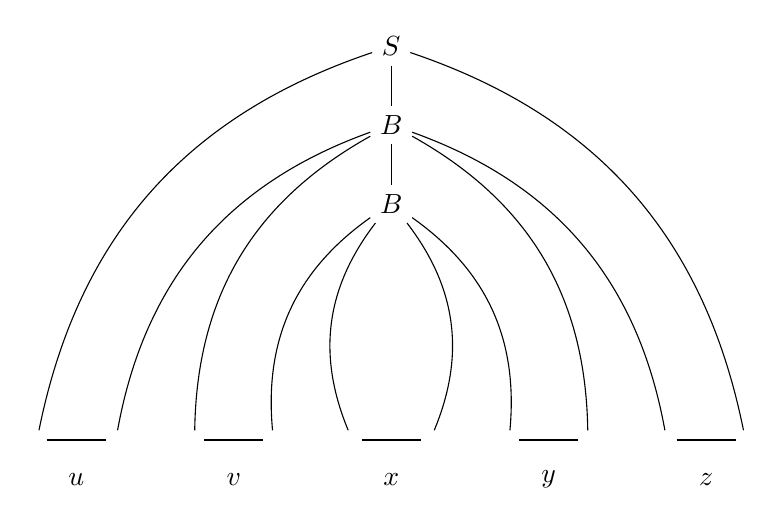
\begin{tikzpicture}[>=latex]
			% Nodes
			\node (u1) at (0,0) {};
			\node (u) at (0.5,-0.5) {$u$};
			\node (u2) at (1,0) {};
			\node (v1) at (2,0) {};
			\node (v) at (2.5,-0.5) {$v$};
			\node (v2) at (3,0) {};
			\node (x1) at (4,0) {};
			\node (x) at (4.5,-0.5) {$x$};
			\node (x2) at (5,0) {};
			\node (y1) at (6,0) {};
			\node (y) at (6.5,-0.5) {$y$};
			\node (y2) at (7,0) {};
			\node (z1) at (8,0) {};
			\node (z) at (8.5,-0.5) {$z$};
			\node (z2) at (9,0) {};

			% Upper nodes
			\node (B2) at (4.5,3) {$B$};
			\node (B1) at (4.5,4) {$B$};
			\node (S) at (4.5,5) {$S$};

			% Lines going down
			\draw[-] (B1) to (B2);
			\draw[-] (S) to (B1);


			% Lines going to terminals
			\draw[-] (B2) to[bend right] (x1);
			\draw[-] (B2) to[bend left] (x2);
			\draw[-] (x1) to (x2);

			\draw[-] (B1) to[bend right] (v1);
			\draw[-] (B2) to[bend right] (v2);
			\draw[-] (v1) to (v2);

			\draw[-] (B1) to[bend left] (y2);
			\draw[-] (B2) to[bend left] (y1);
			\draw[-] (y1) to (y2);

			\draw[-] (B1) to[bend right] (u2);
			\draw[-] (S) to[bend right] (u1);
			\draw[-] (u1) to (u2);

			\draw[-] (B1) to[bend left] (z1);
			\draw[-] (S) to[bend left] (z2);
			\draw[-] (z1) to (z2);

		\end{tikzpicture}
		\caption{\label{fig:pumpelemmacfg} Gentagelse i parsetræ for CFG}
	\end{figure}

	I Figur~\ref{fig:pumpelemmacfg} kan man se hvordan gentagelsen i parsetræet fungerer. Dette betyder naturligvis derfor også at \textbf{både} $v$ og $y$ kan gentages 0 eller flere gange.
\end{proof}



\subsection{Hovedpointer}%
\label{subsec:keypoints}

Disse pointer er taget fra Jørgens \href{https://imada.sdu.dk/u/jbj/DM553/us3.pdf}{Weekly Notes}.

\begin{itemize}
	\item En pushdown automat (PDA) er en nondeterministisk endelig automat forbedret med en stack, som gør PDA'en mere kraftfuld end en DFA eller NFA.
	      \begin{itemize}
		      \item Dette er grundet stakkens uendelige længde. Dog er der stadig begrænsninger, da stakken kører på en LIFO måde.
	      \end{itemize}

	\item If we require that a PDA is deterministic, then we loose power in terms of which languages can be recognized. Note that this did not happen for Finite automata!
	      \begin{itemize}
		      \item Deterministiske PDA'er mister noget kraft, og ud fra Siper's egen forklaring (fra hans kursus på YouTube) er de meget tekniske, men ikke specielt nødvendige for forståelse af automater eller lignende.
	      \end{itemize}
	\item I mentioned the following important fact without proof (see the paper listed under notes on bottom of the homepage) that \textbf{every context-free language over a one-symbol alphabet is also regular.} You are not supposed to be able to prove this, but you must be
	      able to use this fact.
	\item There exist languages that are not context-free, and the pumping lemma can be used to prove that this is the case for a given language. As for regular languages, the proof goes by  contradiction. A typical example of a non-context free language is $\{a^{n}b^{n}c^{n} \; | \; n \ge 0\}$.
	      \begin{itemize}
		      \item Ligesom beskrevet før, er dette fordi stakken ikke er uendeligt kraftfuld, trods dens uendelige længde. Dette er primært grundet dens LIFO måde at agere på.
	      \end{itemize}

	\item Every regular language is context-free
	      \begin{itemize}
		      \item Alle sprog som er regulære er også kontekst-frie. Det vil sige at både endelige automater og pushdown automater kan genkende regulære sprog.
	      \end{itemize}

	\item The class of context free languages is not closed under intersection. Note that this just means that there exists context free languages $L_{1}, L_{2}$ such that $L_{1} \cap L_{2}$ is not context-free. If we take $L_{1} = \{a^{i}b^{j}c^{k}\;|\; i,j,k \ge 0 \text{ and } i = j\}$ and $L_{2} = \{a^{i}b^{j}c^{k}\;|\;i,j,k \ge 0 \text{ and } j = k\}$, then both of these are context-free but $L_{1} \cap L_{2} = \{a^{n}b^{n}c^{n}\; | \; n \ge 0\}$ which we know is not context free.

	      \begin{itemize}
		      \item Det går begge veje. Der eksisterer også \textbf{nogle} snit af kontekstfrie sprog hvis resultat er kontekstfrie. (Specielt givet at alle regulære sprog også er kontekstfri, og snit er lukket under regulære sprog.)
	      \end{itemize}

	\item PDA’s are equivalent to context-free grammars, since, for any PDA A, one can construct a grammar $G$ such that $L(A) = L(G)$, and vice versa.
	      \begin{itemize}
		      \item Dette kan ses i sektion~\ref{subsec:cfgpdaequiv}.
	      \end{itemize}
	\item The class of context-free languages is closed under union, concatenation, and star, but \textbf{not} under intersection and complement. Note that this is NOT the same as saying that the complement of a context-free language is never context free. For example both $\Sigma^{*}$ and its complement, the empty set are context-free (they are also regular). Also $L = \{a^{n}b^{n}\; | \; n \ge 0\}$ and its complement are context-free (but not regular).

	\item The intersection of a context free language $L_{1}$ with a regular language $L_{2}$ is again a context-free language. This can be seen by observing that if we are given a PDA $M_{1}$ for the context-free language $L_{1}$ over $\Sigma$ and a DFA $M_{2}$ for the regular language $L_{2}$, then we can make a PDA $M$ which simulates $M_{1}$ and $M_{2}$ in parallel: think of having pairs of states $(q,p)$ where $q$ is the current state of $M_{1}$ and $p$ is the current state of $M_{2}$. Then on a symbol $a \in \Sigma$ the PDA $M$ will behave as $M_{1}$ in the first coordinate (including updating the stack as $M_{1}$ would) and as $M_2$ in the second coordinate. Now we can make $M$ accept a string $w$ precisely when $M_{1}$ would accept $w$ (be in an accepting state with empty stack AND $M_{2}$ would be in an accepting state after reading $w$). Thus $M$ accepts $w$ if and only if $w \in L_{1} \cap L_{2}$, so $L_{1} \cap L_{2}$ is context-free (as it is accepted by a PDA).

\end{itemize}

%%% Local Variables:
%%% mode: latex
%%% TeX-engine: xetex
%%% TeX-command-extra-options: "-shell-escape"
%%% TeX-master: "main"
%%% End:
